% 第 3 章 §3.5（印刷页 151–162；底本 PDF p.161–p.172）
% 本节无编号公式（第 3 章 (3.1)–(3.8) 全在 §3.1–§3.4）；图 3.8/3.9/3.10/3.13 从略，3.11/3.12 重画。
\usetikzlibrary{patterns}

\section{高维的配边假设}
\label{sec:3.5}

本节所需的那些定义，以及任意维数下配边假设的陈述，现在应当不再那么出人意料了。设 $\mathcal{C}$ 是对称幺半 $(\infty,D)$-范畴；并回忆定义 3.4.9 中的群胚截断 $G_{>k}\mathcal{C}$——它们只保留层次大于 $k$ 的弱可逆态射（可逆性精确到一族相容的高阶同构）。

\begin{definition}[Lurie]
若以下条件成立，则称 $\mathcal{C}$ 中的对象 $x$ 为完全可对偶的（fully dualizable）：(i) 它在 $G_{>1}\mathcal{C}$ 中可对偶；(ii) 其对偶性的单位与迹在 $G_{>2}\mathcal{C}$ 中可对偶；(iii) 上述建立起来的各对偶性的单位与迹在 $G_{>3}\mathcal{C}$ 中可对偶；……（iv）如此继续，直到 $D$-态射——对 $D$-态射我们\emph{不再}要求可对偶。
\end{definition}

停在 $D$ 的理由如下：实现 $D$ 维对偶性的那些态射会落在 $(\infty,D)$-范畴的群胚部分，因而可逆。这又迫使实现对偶性的那些 $D$-态射本身可逆；而向下归纳将迫使所有态射连同 $x$ 一起可逆。可逆的对象固然能给出合法的场论例子，却漏掉了大多数\emph{有趣的}例子。

\begin{theorem}[Lurie, {[19]}]
\begin{enumerate}[label=\arabic*., leftmargin=2.2em, itemsep=0.3em]
\item 函子 $Z\colon\mathsf{Bord}^{\mathrm{fr}}_D\to\mathcal{C}$ 在同构意义下由完全可对偶对象决定，即由正标架点的像 $Z(+)$ 决定。
\item 更精确地说，这类函子连同其自然变换构成的 $(\infty,D)$-范畴是一个群胚，它等价于群胚 $G_{>0}\mathcal{C}$ 中完全可对偶对象所构成的全子群胚。
\item 正交群 $\mathrm{O}(D)$ 通过改变点上 $D$-标架，作用在这类函子 $Z$ 上，从而作用在 $\mathcal{C}$ 中完全可对偶对象构成的空间上。
\item 给定 $D$ 维流形的一个「结构群」$G\to\mathrm{O}(D)$，则 $Z$ 经由切丛上带 $G$-结构的流形所成配边范畴的如下分解
\begin{center}
\begin{tikzcd}[row sep=1.3em, column sep=3.6em]
& \mathsf{Bord}^{G}_D \arrow[dl] \arrow[dr] & \\
\mathsf{Bord}^{\mathrm{fr}}_D \arrow[rr, "Z"'] & & \mathcal{C}
\end{tikzcd}
\end{center}
对应于生成对象 $Z(+)$ 上的 $G$-不动点结构。
\end{enumerate}
\end{theorem}

\begin{remark}[不动点结构]
在 $G$-作用下固定 $Z(+)$，是数据与条件的混合。于是对 $D=1$、$G=\mathrm{O}(1)$，我们需要 $Z(+)$ 上的一个双线性型，它由「与对偶 $Z(-)$ 同构」诱导。图形表明该型必须对称且非退化。

当 $G\to\mathrm{SO}(D)$ 时，$G$-不动点结构是 $\Omega\mathrm{SO}(D)$ 在 $Z(+)$ 上作用的平凡化。于是对 $D=2$、$G=\mathrm{SO}(2)$，$\Omega\mathrm{SO}(2)$ 在 $Z(+)$ 上的作用由 Serre 自同构生成，而不动点信息则是一个同构 $S\cong\mathrm{Id}_{Z(+)}$。
\end{remark}

\subsection{约化到余维 2}

一个对象完全可对偶所需的条件数目，似乎随维数指数式增长；若果真如此，高维中就根本无法利用这个定理。下面我说明情况并非如此：事实上，若忽略标架、只关注定向理论，那么本质上最大的复杂度在 $D=2$ 就已经见到了。这一简化来自三条观察：(i) 所有需要给出的单位、迹态射都对应于配边范畴中的方体；(ii) 所有关系都取「沿公共面粘合两个方体」的几何形式；(iii) 余维大于 $2$ 的一切边界结构都可以忽略。

于是可以假定，我们的态射方体就是手术论中的标准把柄 $D^p\times D^q$，其边界分解为
\[
D^p\times S^{q-1}\ \ \bigsqcup_{S^{p-1}\times S^{q-1}}\ \ S^{p-1}\times D^q .
\]
也就是说，我们面对的是联系两个 $(p+q-1)$-态射的一个 $(p+q)$-态射，而这两个 $(p+q-1)$-态射都从 $\varnothing$ 出发、终止于空集的那个 $(p+q-2)$-自同态 $S^{p-1}\times S^{q-1}$：因此这是一个三层的对象。需要检验的那些对偶关系「$\theta\circ\varepsilon=1$」，将正是手术论中的标准把柄消去关系。

这些观察的后果是：要证明一个对象完全可对偶，只需给出与所有维数不超过 $D$ 的标准把柄相应的 $k$-态射，并检验把柄消去关系。

标架理论需要带标架的把柄。不同的标架相差一个相对于边界而言映入 $\mathrm{SO}(D)$ 的映射，而给出一种表示就得与 $\mathrm{SO}(D)$ 的同伦打交道。这里的信息是有限的，因为组合式的表示只要求找出各同伦群的生成元、检验它们的可逆性，再补上所需的关系。这就增加了「指定一个标架理论」（相对于定向理论而言）在高维中的复杂度。

\subsection{三维的例子}

让我们在三维中演示这些想法，忽略标架、只保留定向。定向范畴格外简单，因为一个态射的伴随总是由反向配边表示，即同一个流形取反定向，再倒过来读作配边（read backwards as a bordims）。（反转标架的约定需要更小心。）回忆上一讲：$\varepsilon\colon\mathrm{Id}\to u\circ ev$ 是 $\Hom(S^0,S^0)$ 中伴随的单位，由一个「拱形」——倒置的马鞍——表示；我将把左伴随 ${}^\vee\varepsilon$ 展示为标准马鞍。配边 $U\colon\mathrm{Id}\to\varepsilon\circ{}^\vee\varepsilon$ 就是莫尔斯理论中熟悉的标准 1-把柄附着，见图 3.8（从略）。

\begin{annote}
底本 p.153 此句印作「read backwards as a bordims」，其中 bordims 应为 bordism；此处照底本排印。
\end{annote}

\figomit{3.8}{由 1-把柄附着所得的配边。}

在定向情形 ${}^\vee\varepsilon=\varepsilon^\vee$；把图倒过来读，就得到相反方向的伴随。迹态射 $T\colon{}^\vee\varepsilon\circ\varepsilon\to\mathrm{Id}$ 是一次 2-把柄附着，如图 3.9（从略）；要看清它，可能需要把连接管拉长，如图 3.10（从略）。

\figomit{3.9}{从 $\varepsilon^\vee\circ\varepsilon$ 到 $\mathrm{Id}$。}
\figomit{3.10}{附着 2-把柄。}

\setcounter{figure}{10}
\begin{figure}[htbp]
\centering
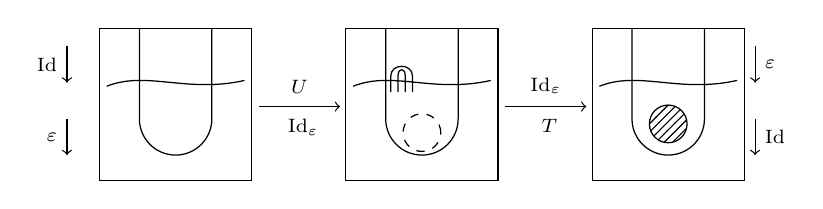
\begin{tikzpicture}[scale=0.92, line width=0.45pt, font=\small]
  % 面板：外框（曲面边界）＋马鞍折痕＋水平的 2-态射带
  \def\panel#1#2{%
    \begin{scope}[shift={(#1,#2)}]
      \draw (0,0) rectangle (2.1,2.1);
      \draw (0.55,2.1) -- (0.55,0.85) arc (180:360:0.5) -- (1.55,2.1);
      \draw (0.10,1.30) .. controls (0.65,1.52) and (1.20,1.20) .. (2.00,1.38);
    \end{scope}}
  \panel{0}{0}
  % 中面板：附着 1-把柄（带电影线的细管），下方虚线圆为新生圆圈
  \panel{3.4}{0}
  \begin{scope}[shift={(3.4,0)}]
    \draw (0.62,1.22) -- (0.62,1.44) .. controls (0.62,1.62) and (0.92,1.62) .. (0.92,1.44) -- (0.92,1.22);
    \draw (0.72,1.22) -- (0.72,1.44) .. controls (0.72,1.56) and (0.82,1.56) .. (0.82,1.44) -- (0.82,1.22);
    \draw[dashed] (1.05,0.66) circle (0.26);
  \end{scope}
  % 右面板：2-把柄的圆盘（斜线填充，原文以蓝色标示）
  \panel{6.8}{0}
  \begin{scope}[shift={(6.8,0)}]
    \fill[pattern=north east lines] (1.05,0.78) circle (0.26);
    \draw (1.05,0.78) circle (0.26);
  \end{scope}
  % 面板之间的复合箭头
  \draw[->] (2.20,1.02) -- (3.32,1.02);
  \node[above, font=\scriptsize] at (2.76,1.06) {$U$};
  \node[below, font=\scriptsize] at (2.76,0.98) {$\boxtimes\ \mathrm{Id}_{\varepsilon}$};
  \draw[->] (5.60,1.02) -- (6.72,1.02);
  \node[above, font=\scriptsize] at (6.16,1.06) {$\mathrm{Id}_{\varepsilon}$};
  \node[below, font=\scriptsize] at (6.16,0.98) {$\boxtimes\ T$};
  % 两端的 1-态射
  \draw[->] (-0.45,1.85) -- (-0.45,1.35) node[midway, left, font=\scriptsize] {$\mathrm{Id}$};
  \draw[->] (-0.45,0.85) -- (-0.45,0.35) node[midway, left, font=\scriptsize] {$\varepsilon$};
  \draw[->] (9.05,1.85) -- (9.05,1.35) node[midway, right, font=\scriptsize] {$\varepsilon$};
  \draw[->] (9.05,0.85) -- (9.05,0.35) node[midway, right, font=\scriptsize] {$\mathrm{Id}$};
\end{tikzpicture}
\caption{「$T\circ U=1$」。（斜线填充的曲面即原文以蓝色标示的 2-态射。）}
\label{fig:3.11}
\end{figure}

图 3.11 说明了关系「$T\circ U=1$」中的一条，即 $(\mathrm{Id}_{{}^\vee\varepsilon}\boxtimes T)\circ(U\boxtimes\mathrm{Id}_{{}^\vee\varepsilon})=\mathrm{Id}_{{}^\vee\varepsilon}$。这就是标准的「用 2-把柄消去 1-把柄」。

\begin{annote}
底本 p.155 此句动词印作 ilustrates，应为 illustrates；译文按正字处理，此处记其原文。
\end{annote}

把图改写成方体形式，可以说明一种归纳式的表述，它使人能把任意维的对偶态射归约为把柄；见图 3.12。图中以蓝色曲面充当 2-态射的那些 1-态射，在首末两图中用黑圈标出：上端是 $u\circ ev$，下端是 $\mathrm{Id}$，二者都从 $S^0=\{+\}\sqcup\{-\}$ 到自身。首末两个「角形马鞍」在配边范畴中表示同一个 2-态射 $\varepsilon$。要插入的两个方体分别表示一次 1-把柄附着及其 2-把柄消去。推广到任意维，只需把顶部的方块 $I\times I$ 换成 $I^p\times I^q$。

\begin{figure}[htbp]
\centering
\begin{tikzpicture}[scale=0.88, line width=0.45pt, font=\small]
  % 立方体（棱长 1.4，进深 0.5）：顶面为充当 2-态射的曲面
  \def\cubebox#1#2{%
    \begin{scope}[shift={(#1,#2)}]
      \fill[pattern=north east lines] (0,1.4) -- (0.5,1.9) -- (1.9,1.9) -- (1.4,1.4) -- cycle;
      \draw (0,0) rectangle (1.4,1.4);
      \draw (0,1.4) -- (0.5,1.9) -- (1.9,1.9) -- (1.4,1.4);
      \draw (1.4,0) -- (1.9,0.5) -- (1.9,1.9);
    \end{scope}}
  % (a) U 形实心曲面
  \begin{scope}[shift={(0,0.35)}]
    \draw (0,0) -- (0,1.6) -- (0.45,1.6) -- (0.45,0.75) -- (1.05,0.75) -- (1.05,1.6) -- (1.5,1.6) -- (1.5,0);
    \draw (1.5,0) -- (1.05,0) -- (1.05,0.35) -- (0.45,0.35) -- (0.45,0) -- cycle;
  \end{scope}
  % (b) 实心立方体
  \cubebox{3.1}{0.35}
  % (c) 附着 1-把柄后的立方体
  \cubebox{6.2}{0.35}
  \begin{scope}[shift={(6.2,0.35)}]
    \draw (0.35,0.45) -- (0.35,0.95) .. controls (0.35,1.20) and (1.05,1.20) .. (1.05,0.95) -- (1.05,0.45);
    \draw (0.62,0.45) -- (0.62,0.95) .. controls (0.62,1.05) and (0.78,1.05) .. (0.78,0.95) -- (0.78,0.45);
  \end{scope}
  % (d) 2-把柄消去后的立方体
  \cubebox{4.65}{-2.15}
  \begin{scope}[shift={(4.65,-2.15)}]
    \fill[pattern=north east lines] (0.35,0.45) rectangle (1.05,0.95);
    \draw (0.35,0.45) rectangle (1.05,0.95);
  \end{scope}
  % 箭头与标注
  \draw[->] (1.75,1.05) -- (2.95,1.05) node[midway, above, font=\scriptsize] {1-把柄附着};
  \draw[->] (4.70,1.05) -- (6.05,1.05);
  \draw[->] (7.95,-0.15) -- (6.30,-1.20) node[midway, right, font=\scriptsize] {2-把柄附着};
  \draw[->] (4.30,-2.50) -- (2.20,-2.50) node[midway, below, font=\scriptsize] {实心立方体};
  \draw[->] (0.75,-0.30) -- (0.75,0.20) node[pos=0, below, font=\scriptsize] {同一个马鞍 $\varepsilon$};
\end{tikzpicture}
\caption{用方体作把柄消去。（斜线填充的曲面即原文以蓝色标示的 2-态射。）}
\label{fig:3.12}
\end{figure}

我们刚画出的方体带有余维 $3$ 的顶点，因此要归约到只含余维 $2$ 角的流形，还需要进一步的论证。完整执行颇为繁复，但想法很简单，并且依赖于归纳地应用配边假设。图 3.13（从略）提示了维数 $3$ 的论证，其中假定 2-对偶性已经检验过，即我们已确立维数不超过 $2$ 的 TQFT 的存在性与相容性。我们沿曲面边界画一个不分段的圆，它把所有把柄附着与消去的步骤都圈在其中。这一步把「带零维角的边界」的细分或重组分离到理论的二维部分，并表明三维理论中的运算与关系可以只在以圆为边界的曲面上定义和检验。

\figomit{3.13}{无需角。}

\begin{remark}
回忆莫尔斯理论：任何流形都可以从空集出发、通过附着把柄造出，而所有运算只涉及带余维 $2$ 角的流形。初看之下，这似乎暗示存在一种只深入两层的 TQFT 分类，从而完全避开 $2$ 以上的范畴。事实上，这个方向在三维确有一个部分结果，即 Reshetikhin--Turaev 定理 [25]：它分类了「两层深」的三维 TQFT，其联系于圆周的范畴半单。然而超过三维就没有希望了：用于附着把柄的球面可能以复杂的方式嵌入。例如，单连通可微四维流形的全部复杂性，都隐藏在三维流形的链环理论里，而后者正是用来附着 2-把柄的。尽管如此，这一观察仍然有用：如果我们能把各边界本身、以及边界的进一步边界，都切成把柄，那么这种「余维 2」的直觉就变成正确的，并发展为只用标准把柄与消去来检验可对偶性的递归程序。
\end{remark}

\subsection{张量范畴与模范畴}

现在我们转向配边假设的一个三维演示，它使构造有趣的三维 TQFT 成为可能。关键例子来自 Douglas、Schommer-Pries 与 Snyder 的近期工作。\footnote{作者非常感谢他们的解释，那远在该文公开面世之前。}

我们把张量范畴（tensor category）$\mathcal{T}$ 定义为一个带双线性幺半结构的线性范畴。\footnote{有些文献，例如 [9]，还附加了额外的条件。}回忆一个小麻烦：张量积的结合性由一个结合子
\[
\alpha_{x,y,x}\colon (x\otimes y)\otimes z\xrightarrow{\ \sim\ }x\otimes(y\otimes z)
\]
调节，它服从 Stasheff 的五边形恒等式。不过我们很走运，因为 MacLane 的相干定理允许把 $\mathcal{T}$ 换成一个结合性严格的等价范畴。

\begin{annote}
底本 p.157 此处印作 $\alpha_{x,y,x}$，而所论的张量积为 $(x\otimes y)\otimes z$，故第三个下标应为 $z$；此处照底本排印。
\end{annote}

$\mathcal{T}$ 上的一个模范畴（module category）$\mathcal{M}$，是一个带双线性乘法函子 $\mathcal{T}\times\mathcal{M}\to\mathcal{M}$ 的线性范畴，并满足定义 $\mathcal{T}$ 在 $\mathcal{M}$ 上作用所需的那些显然的约束。（同样可以证明，我们可以修改 $\mathcal{M}$，得到一个严格模范畴，其中各相干同构都是恒等；见 [16]。）

\subsection{范畴的张量积}

阿贝尔范畴情形的定义（属于 Deligne）借自代数：对右 $\mathcal{T}$-模 $\mathcal{M}$ 与左 $\mathcal{T}$-模 $\mathcal{N}$，$\mathcal{M}\boxtimes_{\mathcal{T}}\mathcal{N}$ 是这样一个范畴，它余表示那个把线性范畴 $\mathcal{C}$ 送到「$\mathcal{T}$-双线性、右正合双函子 $\mathcal{M}\times\mathcal{N}\to\mathcal{C}$ 构成的范畴」的函子。然后可以证明，阿贝尔范畴的张量积可由某个阿贝尔范畴余表示；见 [16]。

\begin{remark}
阿贝尔范畴在 $\mathsf{Vect}$ 上的张量积已经有些微妙：例如 $\mathcal{M}\boxtimes_{\mathsf{Vect}}\mathcal{N}$ 的对象比单纯的直和 $m\boxtimes n$（$m\in\mathcal{M}$、$n\in\mathcal{N}$）要多；我们必须对商（余核）封闭。所得的范畴是阿贝尔的。若 $\mathcal{M}$、$\mathcal{N}$ 分别是 $A$-模与 $B$-模范畴，则 $\mathcal{M}\boxtimes\mathcal{N}$ 是 $(A\otimes B)$-模范畴。
\end{remark}

这些定义的要点，应当是构造一个（弱的）对称幺半 3-范畴：以张量范畴为对象，以双模范畴为态射，以张量积为合成，以双模函子为 2-态射，最后以它们之间的自然变换为 3-态射。构造的某些成分已在 [16] 中写出；完整的细节见近期的文章 [8]。

\begin{definition}
若每个对象都有左对偶与右对偶，则称张量范畴是刚性的（rigid）。把一个对象送到它的左对偶、右对偶，定义了 $\mathcal{T}$ 上两个反变函子；它们互为逆。刚性张量范畴有一些格外好的性质 [9]；特别地，若 $\mathcal{T}$ 是阿贝尔的，则乘法 $\otimes\colon\mathcal{T}\times\mathcal{T}\to\mathcal{T}$ 是双正合的，内部对偶函子也是。
\end{definition}

\subsection{2-可对偶性}

每个张量范畴 $\mathcal{T}$ 都是 1-可对偶的，其对偶是乘法反向范畴 $\mathcal{T}^{\mathrm{mo}}$，即同一范畴取相反的张量积。其论证重复代数的情形，而 $u$、$ev$ 由 $\mathcal{T}$ 作为 $\mathcal{T}^e$-模来表示。

我们也可以摹仿 §3.4 中关于 2-对偶性的代数计算。这里需要 $\mathcal{T}$ 作为线性范畴可对偶，并且作为 $\mathcal{T}^e$-模可对偶。Serre 函子是 $\mathcal{T}$ 作为线性范畴的对偶，我们把它记作 $\mathcal{T}^\vee$。2-可对偶性要求它是一个可逆双模，且其逆必须是（右正合）函子构成的双模范畴 $\Hom_{\mathcal{T}^e}(\mathcal{T};\mathcal{T}^e)$。此外，与 $\mathcal{T}$ 在 $\mathcal{T}^e$ 上作张量积应当是范畴上的正合运算（与有限滤过极限、余极限交换）。

我们可以更精确地识别 $\mathcal{T}^\vee$。若 $\mathcal{T}$ 中所有对象都紧——例如诺特环上有限生成模的范畴就是如此——则 $\mathcal{T}^\vee$ 可以等同于线性反向范畴 $\mathcal{T}^\circ$，办法是把对象 $a^\circ\in\mathcal{T}^\circ$ 送到余表示函子 $x\mapsto\Hom(a,x)$。我们将在下文定理 3.5.13 之后、在刚性范畴的特殊情形里，进一步写出 $\mathcal{T}^\vee$ 的更多结构。

\subsection{Drinfeld 中心与 Hochschild 同调}

与闭 1-流形相联系的是线性范畴；而与标架圆周 $S^1_n$（$n>0$）相联系的，是张量积 $\mathcal{T}\otimes_{\mathcal{T}^e}(\mathcal{T}^\vee)^{\otimes_{\mathcal{T}}(n-1)}$，其中 $(\mathcal{T}^\vee)^{\otimes_{\mathcal{T}}(n-1)}:=\mathcal{T}^\vee\otimes_{\mathcal{T}}\cdots\otimes_{\mathcal{T}}\mathcal{T}^\vee$ 是 Serre 双模 $\mathcal{T}^\vee$ 的 $(n-1)$ 次幂。$n\le 0$ 情形的描述涉及 $\mathcal{T}^\vee$ 的逆双模，但另一种表述利用 $\mathcal{T}$ 在 $\mathcal{T}^e$ 上的可对偶性，把带逆幂的张量积改写成 Hom-范畴。确切地说，$n\le 0$ 时的范畴是 $\Hom_{\mathcal{T}^e}\bigl((\mathcal{T}^\vee)^{\otimes_{\mathcal{T}}(-n)},\mathcal{T}\bigr)$。这里 Hom 指与 $\mathcal{T}^e$-作用相容的、线性的右正合函子构成的范畴。与代数的情形不同，与 $\mathcal{T}$-作用的相容性带有数据，而不只是条件；我们马上会在例子中看到这一点。

0-标架圆周对应的范畴 $\Hom_{\mathcal{T}^e}(\mathcal{T},\mathcal{T})$ 地位特殊，因为它在合成下带有自然的张量结构。它等价于 $\mathcal{T}$ 的 Drinfeld 中心（Drinfeld center）$\mathcal{DC}(\mathcal{T})$：这是由对 $(x,\beta)$ 构成的范畴，其中 $x\in\mathcal{T}$，而 $\beta$ 是与 $x$ 的半编织（half braiding），即函子 $x\otimes$ 与 $\otimes x$（分别用 $x$ 左乘与右乘）之间的一个乘法性同构。读者大概能猜出 $\beta$ 的乘法性是什么意思，只要参照编织的条件（§3.3）：那就是三角形的交换性
\begin{center}
\begin{tikzcd}[row sep=1.9em, column sep=4.4em]
& y\otimes x\otimes z \arrow[dl, "\beta(y)\otimes\mathrm{Id}_z"'] \arrow[dr, "\mathrm{Id}_y\otimes\beta(z)"] & \\
x\otimes y\otimes z \arrow[rr, "\beta(y\otimes z)"'] & & y\otimes z\otimes x
\end{tikzcd}
\end{center}

Drinfeld 中心带有自然的编织 $\beta(x,y)\colon x\otimes y\xrightarrow{\sim}y\otimes x$，它来自第一个对象 $x$ 所携带的半编织。这个编织通常不是对称的。

\begin{remark}
实践中，编织力求「极大程度地非对称」。例如，若 $\mathcal{T}$ 是有限阿贝尔群 $F$ 的表示张量范畴 $(\mathrm{Rep}(F),\otimes)$（在 $\C$ 上作张量积），则其中心是 $F\times F^\vee$ 的表示张量范畴，但带有由 $F$、$F^\vee$ 映入 $\C^\times$ 的自然配对所定义的、类似 Heisenberg 的非退化编织。

具体地说，记 $n=\#F$，由 Pontrjagin 配对映入 $\mu_n\subset\C^\times$ 诱导出 $H^4(B^2F\times B^2F^\vee;\mu_n)$ 中一个特殊类。把它当作 $k_3$-不变量，就为我们造出一个 $\pi_2=F\times F^\vee$、$\pi_3=\mu_n$ 的空间。于是我们按命题 3.3.14 构造一个编织张量范畴。这个张量范畴按 $\mu_n$ 的特征标分裂为 Fourier 分量。对应于标准特征标的那个直和项，同构于 $(\mathrm{Rep}(F),\otimes)$ 的 Drinfeld 中心。

更一般地，任何有限群 $G$ 都有「范畴化的群环」，即 $G$ 上向量丛的范畴，其张量结构来自卷积。这是群上函数的显然范畴类比。它的 Drinfeld 中心是 $G$ 上 $G$-等变向量丛的张量范畴，带卷积结构与一个有趣的编织。这是 $G$ 上类函数的范畴化类比。上一例中 $G=F^\vee$。
\end{remark}

\begin{remark}
在 3-可对偶的情形，Serre 函子的平方是恒等，因为 $\pi_1\mathrm{SO}(3)=\Z/2$；因此与圆周上两个 3-标架 $S^1_{\mathrm{even}}$ 和 $S^1_{\mathrm{odd}}$ 相配的范畴只有两个，即 $\mathcal{DC}(\mathcal{T})=\Hom_{\mathcal{T}^e}(\mathcal{T},\mathcal{T})$ 与 $\mathcal{T}\otimes_{\mathcal{T}}\mathcal{T}$。
\end{remark}

\subsection{融合范畴}

以张量范畴为基础的三维扩展 TQFT，并没有一个像二维那样（用半单、不必交换的代数）的完整分类。存在一些约束；例如当 $\mathcal{T}$ 是阿贝尔时，完全可对偶性要求 Drinfeld 中心（及其扭转形式，即 Hochschild 同调）半单。这可由 TQFT 中一个重要运算——维数约化（dimensional reduction）——的特殊情形推出。此时我们沿 $S^1$ 约化由 $\mathcal{T}$ 生成的三维 TQFT $Z_{\mathcal{T}}$，得到二维理论 $S^1\backslash Z_{\mathcal{T}}$，它由 $S^1\backslash Z_{\mathcal{T}}(M):=Z_{\mathcal{T}}(M\times S^1)$ 定义；这个理论必须由 $S^1\backslash Z_{\mathcal{T}}(+)=Z_{\mathcal{T}}(S^1)$ 生成，于是 $\mathcal{DC}(\mathcal{T})$ 半单。

中心的半单性对刚性范畴是自动的，但一般来说是很强的约束。

\begin{exercise}
计算「$\mathsf{Vect}$ 上 $2\times 2$ 上三角矩阵代数」的 Drinfeld 中心，即范畴 $\mathsf{Vect}^{\oplus3}$，其张量积摹仿矩阵 $\left[\begin{smallmatrix}a&b\\0&c\end{smallmatrix}\right]$ 的乘法。
\end{exercise}

然而，一类漂亮的扩展三维 TQFT 来自 Douglas、Schommer-Pries 与 Snyder 的下述结果。它基于融合范畴（fusion category）这一概念，后者已是大量研究的对象（Etingof、Ocneanu 等）。与二维故事在措辞上的相似有些误导：融合范畴的结构比复半单代数的结构复杂得多。

\begin{definition}
融合范畴是只有有限多个单对象同构类的半单刚性张量范畴。
\end{definition}

\begin{example}
有限群 $G$ 的范畴化群环；见注 3.5.7。它生成以有限群 $F$ 为规范群的三维规范理论。张量结构、以及由此得到的 TQFT，可以用一个余圈 $\tau\in H^3(BF;\C^\times)$ 扭转——这是「用 $\C^\times$ 对群作中心扩张」的高维类比，后者在二维生成规范理论的扭转版本。在张量范畴中，该余圈表现为结合子。

单位根处量子群（quantum group）表示的半单化范畴（即有限维表示的范畴，模去量子维数为零的表示）。与之相伴的三维场论计算 Turaev--Viro 理论，其闭三维流形不变量是著名的 Chern--Simons 不变量的平方范数。\footnote{目前，对一般的非阿贝尔 $G$，还没有在全扩张 TQFT 之内构造 Chern--Simons 不变量的办法，尽管 Bartels、Henriques 与 Douglas 的一个方案已接近完成。然而，生成它的张量范畴类比远非离散，而是用 von Neumann 代数描述的。对环面群，可以落在拓扑范畴中，并出现一个 $C^*$ Hopf 式的代数，[11]。}
\end{example}

这些条件强到足以推出张量积运算的良好行为。

\begin{theorem}[Etingof--Nykshich--Ostrik]
对融合范畴 $\mathcal{F}$ 上任意右半单与左半单的模范畴 $\mathcal{M}$、$\mathcal{N}$，张量积 $\mathcal{M}\boxtimes_{\mathcal{F}}\mathcal{N}$ 半单。它还对 $\mathcal{M}$ 与 $\mathcal{N}$ 正合。
\end{theorem}

\begin{annote}
底本 p.161 与 p.162 两处均印作「Etingof--Nykshich--Ostrik」，而本章文献 [9]、[10] 作 Nikshych；此处照底本排印，应为 Etingof--Nikshych--Ostrik。
\end{annote}

于是我们可以定义融合范畴的一个「小」3-范畴：对象为融合范畴，态射为半单双模范畴，2-态射为函子，3-态射为自然变换。在融合范畴的框架里，我们还有一对对偶性，使张量积可以解释为函子范畴。特别地，这确立了 Drinfeld 中心及其扭转形式的半单性。

\begin{theorem}[Douglas--Schommer-Pries--Snyder, {[8]}]
每个融合范畴 $\mathcal{F}$ 都是 3-范畴 $\mathcal{T}\mathsf{cat}$ 中的完全可对偶对象。特别地，它定义一个标架 TQFT $Z_{\mathcal{F}}\colon\mathsf{Bord}^{\mathrm{fr}}_3\to\mathcal{T}\mathsf{cat}$。范畴 $Z_{\mathcal{F}}(S^1_0)$ 是 $\mathcal{F}$ 的 Drinfeld 中心，带其自然张量结构。Serre 函子是 $\mathcal{F}$ 中的双对偶函子。
\end{theorem}

由于 $\pi_1\mathrm{SO}(3)=\Z/2$（而不再是 $\Z=\pi_1\mathrm{SO}(2)$），任何 3-可对偶对象的 Serre 自同构必须平方为 $1$。作为推论，作者们得到了关于融合范畴的一个近期结果 [10] 的富有启发的证明，而后者又基于 Radford 更早的工作 [24]。

\begin{corollary}[Etingof--Nykshich--Ostrik]
在任何融合范畴中，四重对偶函子与恒等函子之间有典范同构。
\end{corollary}

\subsection{Serre 自同构 $\mathcal{T}^\vee$}

让我们在刚性情形下写出「Serre 函子等同于双右对偶函子」这一识别。它并不依赖 $\mathcal{T}$ 的半单性。回到 §3.5.5 中的等同 $\mathcal{T}^\circ=\mathcal{T}^\vee$：它把 $a^\circ\in\mathcal{T}^\circ$ 送到泛函 $X\mapsto\Hom_{\mathcal{T}}(a,X)$。我断言 $x\otimes a^\circ\otimes y=(y^\vee\otimes a\otimes{}^\vee x)^\circ$，因为对泛函 $X\mapsto F(X)$ 有 $(x\otimes F)(X)=F(X\otimes x)$；据此，我们可以使用 ${}^\vee x$、$y^\vee$ 的 Hom-对偶性质：
\[
\Hom_{\mathcal{T}}(a,y\otimes X\otimes x)=\Hom_{\mathcal{T}}(y^\vee\otimes a\otimes{}^\vee x,X).
\]
现在用右对偶把 $\mathcal{T}$ 与 $\mathcal{T}^\circ$ 等同起来：$a\mapsto(a^\vee)^\circ$。上述关系于是变为
\[
x\otimes(a^\vee)^\circ\otimes y=(y^\vee\otimes a^\vee\otimes{}^\vee x)^\circ
=\Bigl[\bigl({}^{\vee\vee}x\otimes a\otimes y\bigr)^\vee\Bigr]^\circ .
\]
结果是把 Serre 双模 $\mathcal{T}^\vee$ 识别为 $\mathcal{T}$，但左张量作用被双左对偶扭转。这就是双左对偶函子的双模实现。

\begin{remark}
若 $S$ 不同构于 $\mathrm{Id}$，则该 TQFT 可以对 Spin 曲面定义。若双对偶同构于恒等，则称刚性范畴是枢轴的（pivotal）。在融合情形，枢轴结构使我们能从 Spin 曲面过渡到定向曲面。进一步走到三维流形，为了从标架情形过渡到定向情形，我们需要所谓球状结构（spherical structure）：即一个枢轴结构，其中「Serre（双对偶）的平凡化」的平方等于「四重对偶的典范平凡化」。

「Serre 应当是张量函子、而不只是双模范畴」这一条件，与内部对偶的存在密切相关：$(\mathcal{F}-\mathcal{F})$-双模 $\mathcal{S}$ 恰好在 $\mathcal{S}$ 分别作为左 $\mathcal{F}$-模与右 $\mathcal{F}$-模都等价于 $\mathcal{F}$ 时，才由某个张量自同构实现。它所实现的张量自同构，就是这些各自「拉直」的同构的复合。在刚性情形，$\mathcal{F}$ 与 $\mathcal{F}^\vee$ 之间的两个拉直同构都是内部对偶函子。
\end{remark}
